\section*{Results}

\subsection*{Observed CoSMoS data} % Figure 1B,C,D

To maximize the extraction of useful information from data we use full 2-D images for analysis. For co-localization analysis it is sufficient to analyze the image area local to the target molecule. The area of interest (AOI) analyzed needs to be large enough so that fluorescence spots can be clearly distinguished from background, allowing  reliable  determination of the  local  background  intensity. Typical half-width of fluorescence spots in experiments used in this work is 1-2 pixels and therefore we chose the size of AOI to be 14x14 pixels (Figure 1C,D). In addition to AOIs centered at target molecules, it is useful to also collect AOI images from randomly selected sites at which no target molecule is present as a negative control data (Figure 1D). Such off-target control data is analyzed jointly with on-target data and serves to facilitate the estimation of the background level of nonspecific binding. Construction of CoSMoS data for Tapqir includes localization of target molecules in the target channel, registration of target and binder channels, and time-dependent drift correction and can be performed with any existing tools \cite{Friedman2015-nx, Smith2019-yb} (Figure 1B).

 % One experiment typically consists of a set of images where we have $N$ target sites ($n \in \{1,\dots,N\}$) each consisting of a series of $F$ different images in a recording ($f \in \{1,\dots,F\}$) (a “recording”).

\subsection*{Bayesian image classification analysis}

To solve the problems with existing CoSMoS data analysis identified above, we developed a new method that is accurate, objective, and built on a rigorous Bayesian statistical approach to the CoSMoS image analysis problem. To perform a Bayesian analysis of the data one must 1) define the model for the observed data in terms of model parameters, 2) specify priors for random model parameters, and 3) specify the likelihood for the observed data given the model. Our CoSMoS model classifies the observed images using a probabilistic mixture formalism that includes spots from both specifically and non-specifically bound molecules. Specification of priors for random model parameters allows us to embed our knowledge about the experiment (e.g., the likely positions of specifically and non-specifically bound molecules). Our likelihood function takes the idealized image model and incorporates physically realistic photon shot-noise. Inference of model parameters and classification of images is summarized in posterior distributions which are calculated using Bayes' rule. The analysis is “time-independent”, meaning that we ignore the time dimension of the recording -- the order of the images does not affect the model, as each image is considered statistically independent of the others. 

\subsection*{Model} % Figure 2A,B,C

A single AOI image from a CoSMoS dataset is a matrix of noisy pixel intensity values centered at the location of a target molecule. In each image, multiple binder molecules can be present. Figure 2A shows an example image where two spots are present, one spot is located near the target molecule at the center of the AOI and another is off-target. We model an AOI image as a constant average background intensity $b$ summed with fluorescence spots modeled as 2-D Gaussians $\mu^S$, which accurately approximate the microscope point spread function \cite{Zhang2007-rb} (Figure 2B). The spots are numbered and each Gaussian is parameterized by integrated intensity $h$, width $w$, and position $x$ and $y$ relative to the AOI center. For the data we typically encounter, there are no more than two spots present in a single AOI. We therefore use $K$ = 2 as the default maximum  number of spots per AOI in all analyses presented here. The presence or absence of each spot is denoted by a binary indicator parameter $m \in \{0, 1\}$. The resulting mixture model has four possible combinations for $m_1$ and $m_2$: (1) a “no-spot” image that contains only background (Figure 2B, top left), (2) a single “spot” image that contains the first binder molecule spot superimposed on background (Figure 2B, bottom left), (3) a single “spot” image that contains the second binder molecule spot superimposed on background (Figure 2B, top right), and (4) a two-spot image that contains two binder molecule spots superimposed on background (Figure 2B, bottom right).  % We assume that background and spots have Gaussian noise. (Improvement of the preliminary method to include more realistic noise models is proposed in Aim 1a.)  each spot image is modelled as a Gaussian perturbation of the sum of the background λae treat the image recording using a standard likelihood “mixture model”71, in which the data are considered a mixture of spot and background images of unknown proportions. Frequently, identification of on-target binding is complicated by molecules binding off-target which distort the shape of the on-target spot and its apparent distance to the target. In addition to the on-target spot, non-specifically bound binder molecules can also be present in the image. Unlike on-target binding, nonspecific interaction can be anywhere in the image.

Among the spots that are present in an AOI, by assumption at most only one can be bound specifically. To classify spots as specific or non-specific we introduce the index parameter $\theta \in \{0,1,\dots,K\}$. $\theta$ uniquely determines the index of the specifically bound molecule when it is present (Figure 2C, middle and right) and equals zero when it is absent (Figure 2C, left). Since negative control AOIs which are not centered on target molecules contain only non-specific binding, we set $\theta = 0$ for all control data images. 

\subsection*{Parameter priors}

Specifying parameter priors is essential for Bayesian analysis and allows us to incorporate existing experimental knowledge. For most model parameters, there is no strong prior information so we use uninformative priors (see Methods). However, we have strong expectations for the positions of specific and non-specific binder molecules that can be expressed as prior distributions and used effectively to discriminate between the two. Non-specific binding can occur anywhere on the surface with equal probability and thus has a uniform prior distribution across the image. Specific binding, on the other hand, is co-localized with the target molecule and has a prior distribution peaked at the target location (Supplementary Figure 2). % [The width of the prior distribution for specific binding location depends on multiple experiment characteristics such as the spot localization accuracies and the mapping accuracy between target and binder channels.]

[Hyperpriors, some are learned from the data] Parameters $\theta$ and $m$ depend  hyperpriors 

Specific and non-specific binding also have different binding frequencies. For example, increasing the ratio of the non-specific to specific binding frequencies decreases the probability of the spot being classified as specific. %  Thus, there are total $2^K + K2^{K-1}$ unique combinations of $\mathrm{m}$ and $\theta$ which define the state space for mixture model. The probability of being on-target or off-target is dictated primarily by the distance to the target.

\subsection*{Intensity model (likelihood function)}

Total observed intensity $D$ is the sum of the image model perturbed by the shot-noise and the offset signal $\delta$ (dark current). The linear relationship between the noise variance and the mean intensity is built into the intensity model through the gain and offset parameters and the gain parameter is fitted along with other parameters. Distribution of the offset signal is obtained as a histogram density signal from the single-molecule images.

% p(x,y|theta) p(theta|pi) p(m | pi, lambda) p(pi| _) p(lambda| _)

\subsection*{Generative model} % Figure 2D

The probabilistic model can be interpreted as a generative process that produces the observed image data. A graphical model describing the structure of probabilistic relationships in the model is shown in Figure 2C. In this directed graph, nodes are either random variables (circles) or deterministic functions (diamonds). Related nodes are connected by edges, with an arrow pointing towards the dependent variable. The shape of the 2-D Gaussian spot $\mu^S$ depends on spot variables ($h, w, x, y$) and the noiseless image shape $\mu^I$ is the sum of background intensity $b$ and spot images $\mu^S$. A dashed box represents activation of spot variables based on the spot existence indicator. Finally, plates represent replication and specify an index for the repeated variable. As was mentioned above, frames are treated as being time-independent. 
%[The probabilistic model described above is versatile and allows to capture many of the characteristics of real experimental data, such as site and time dependent fluctuations in the local background signal, time dependent fluctuations in the spot intensity and its position, simultaneous presence of on-target and off-target spots, photon shot-noise modeled as a Gamma distribution, which is more realistic than Gaussian noise.]


\subsection*{Bayesian Inference and Implementation}

Posterior distributions of latent variables conditioned on the observed data is obtained by using Bayes' theorem. The evidence term (marginal likelihood) in Bayes' theorem in general is intractable. Here we use stochastic variational inference (SVI) approach and maximize the evidence-lower bound (ELBO). The model and the SVI of model parameters were implemented as a probabilistic program, Tapqir, in the Python-based probabilistic programming language (PPL) Pyro. The advantage of using PPL like Pyro is its black box SVI approach which allows to focus on the model development, efficient computation on GPU, scalability to large datasets. Details of the generative model and variational model are given in the online Methods section.

However, it is not necessary to measure the width; with enough data the algorithm can learn its value from the data.  These parameters are learned from the data and both affect the posterior probabilities of a spot being classified as specific or non-specific.

\subsection*{Tapqir analysis} % Figure 3

To demonstrate the application of Tapqir, we used simulated data with high SNR and noisy experimental data with low SNR. Briefly, we simulated time-independent single-molecule co-localization dataset consisting of 2500 on-target data images and 2500 control data images that mimics high quality data (SNR = 3.76) with average specific binding probability 0.15 and non-specific binding rate 0.15. Noisy experimental data is taken from another work [short description and reference]. For each dataset on-target and control data were analyzed jointly. Figure 3 show short extract of analysis results for the simulated data (Figure 3A) and for the experimental data (Figure 3B). Cartoons above the images summarize analysis results and show only molecules with probability higher than 0.5 and their most likely position. Plots below the images in each panel show mean values and confidence intervals of inferred model parameters for each spot. The program additionally calculates the probability that an specifically bound molecule is present (green) and that at least one non-specifically bound molecule is present (red) in each frame of the recording at every target molecule location. Tapqir correctly detects specifically bound spots (p, green curve, e.g. frame 170 in A and frame 635 in B) and non-specifically bound spots (p, red curve, e.g. frame 173 in A and frame 635 in B). The program estimates spot parameters in a meaningful manner. For example, high intensity spots are classified as specific if located near the target molecule and non-specific if located off-target. When the spot is absent it has a near zero intensity and high position uncertainty meaning it cannot be localized. Apart from these two extreme scenarios intermediate cases can also be observed in the noisy experimental data. The program also determines background intensity for each image. % (change the color). Talk about the possibility of spots being partially present for the duration of a single frame in experimental data

\subsection*{Tapqir performance on simulated data} % Figure 4

Next, to validate Tapqir we tested its performance on simulated data. Synthetic-data simulation is important because it allows to directly check that the inference spot classification is reliable for a wide range of model parameters. To test the classification accuracy we made three types of simulations: 1) synthetic datasets with varying SNR, 2) simulations with varying non-specific binding rate, and 3) simulations with no specific binding and varying rate of non-specific binding. Figure 4A shows examples of images with different SNR for illustration purposes. We made 10 randomized simulations and then fit the synthetic data to the model. Figure 3 shows plots of the simulated values of the global parameters (gain, average on-target spot probability, average off-target spot probability, proximity) vs the fitted values. The results demonstrate that model parameters can be reliably recovered which is good.

By analyzing simulated data we have established that this parameter, also called the proximity parameter, can be reliably determined by floating it during the fit (Figure ). Alternatively, proximity parameter can be determined experimentally and fixed in the model. Figure show the distribution of the center of mass of on-target spots which are tightly clustered around the target molecule. On the other hand, off-target spots are distributed more uniformly across the area of the image.

This standard distribution can be determined independently and used as a fixed parameter in the model. However, it can also be floated in the fit and determined from the overall distribution of the center of masses of spots. $\sigma^{xy}$, $\pi^z$, and $\lambda^j$ are correlated. Figure shows simulated data with varying parameters where the true values of parameters are inferred correctly. Note that the posterior probability of the spot class depends on its relative position to the target and average probabilities of on-target and off-target spots.

In Figure we show raw images and their intensity distributions along with the images simulated from the posterior distribution (posterior predictive checking). Comparison of images and distributions for spot/no spot cases show that our model accurately models intensity as a function of mean intensity reflecting the dependence of the noise on the mean intensity. Additionally, Figure shows that the gain parameter is accurately inferred for a simulated set of data with varying gain parameter where the true value of the gain parameter is known.

%\begin{figure}
%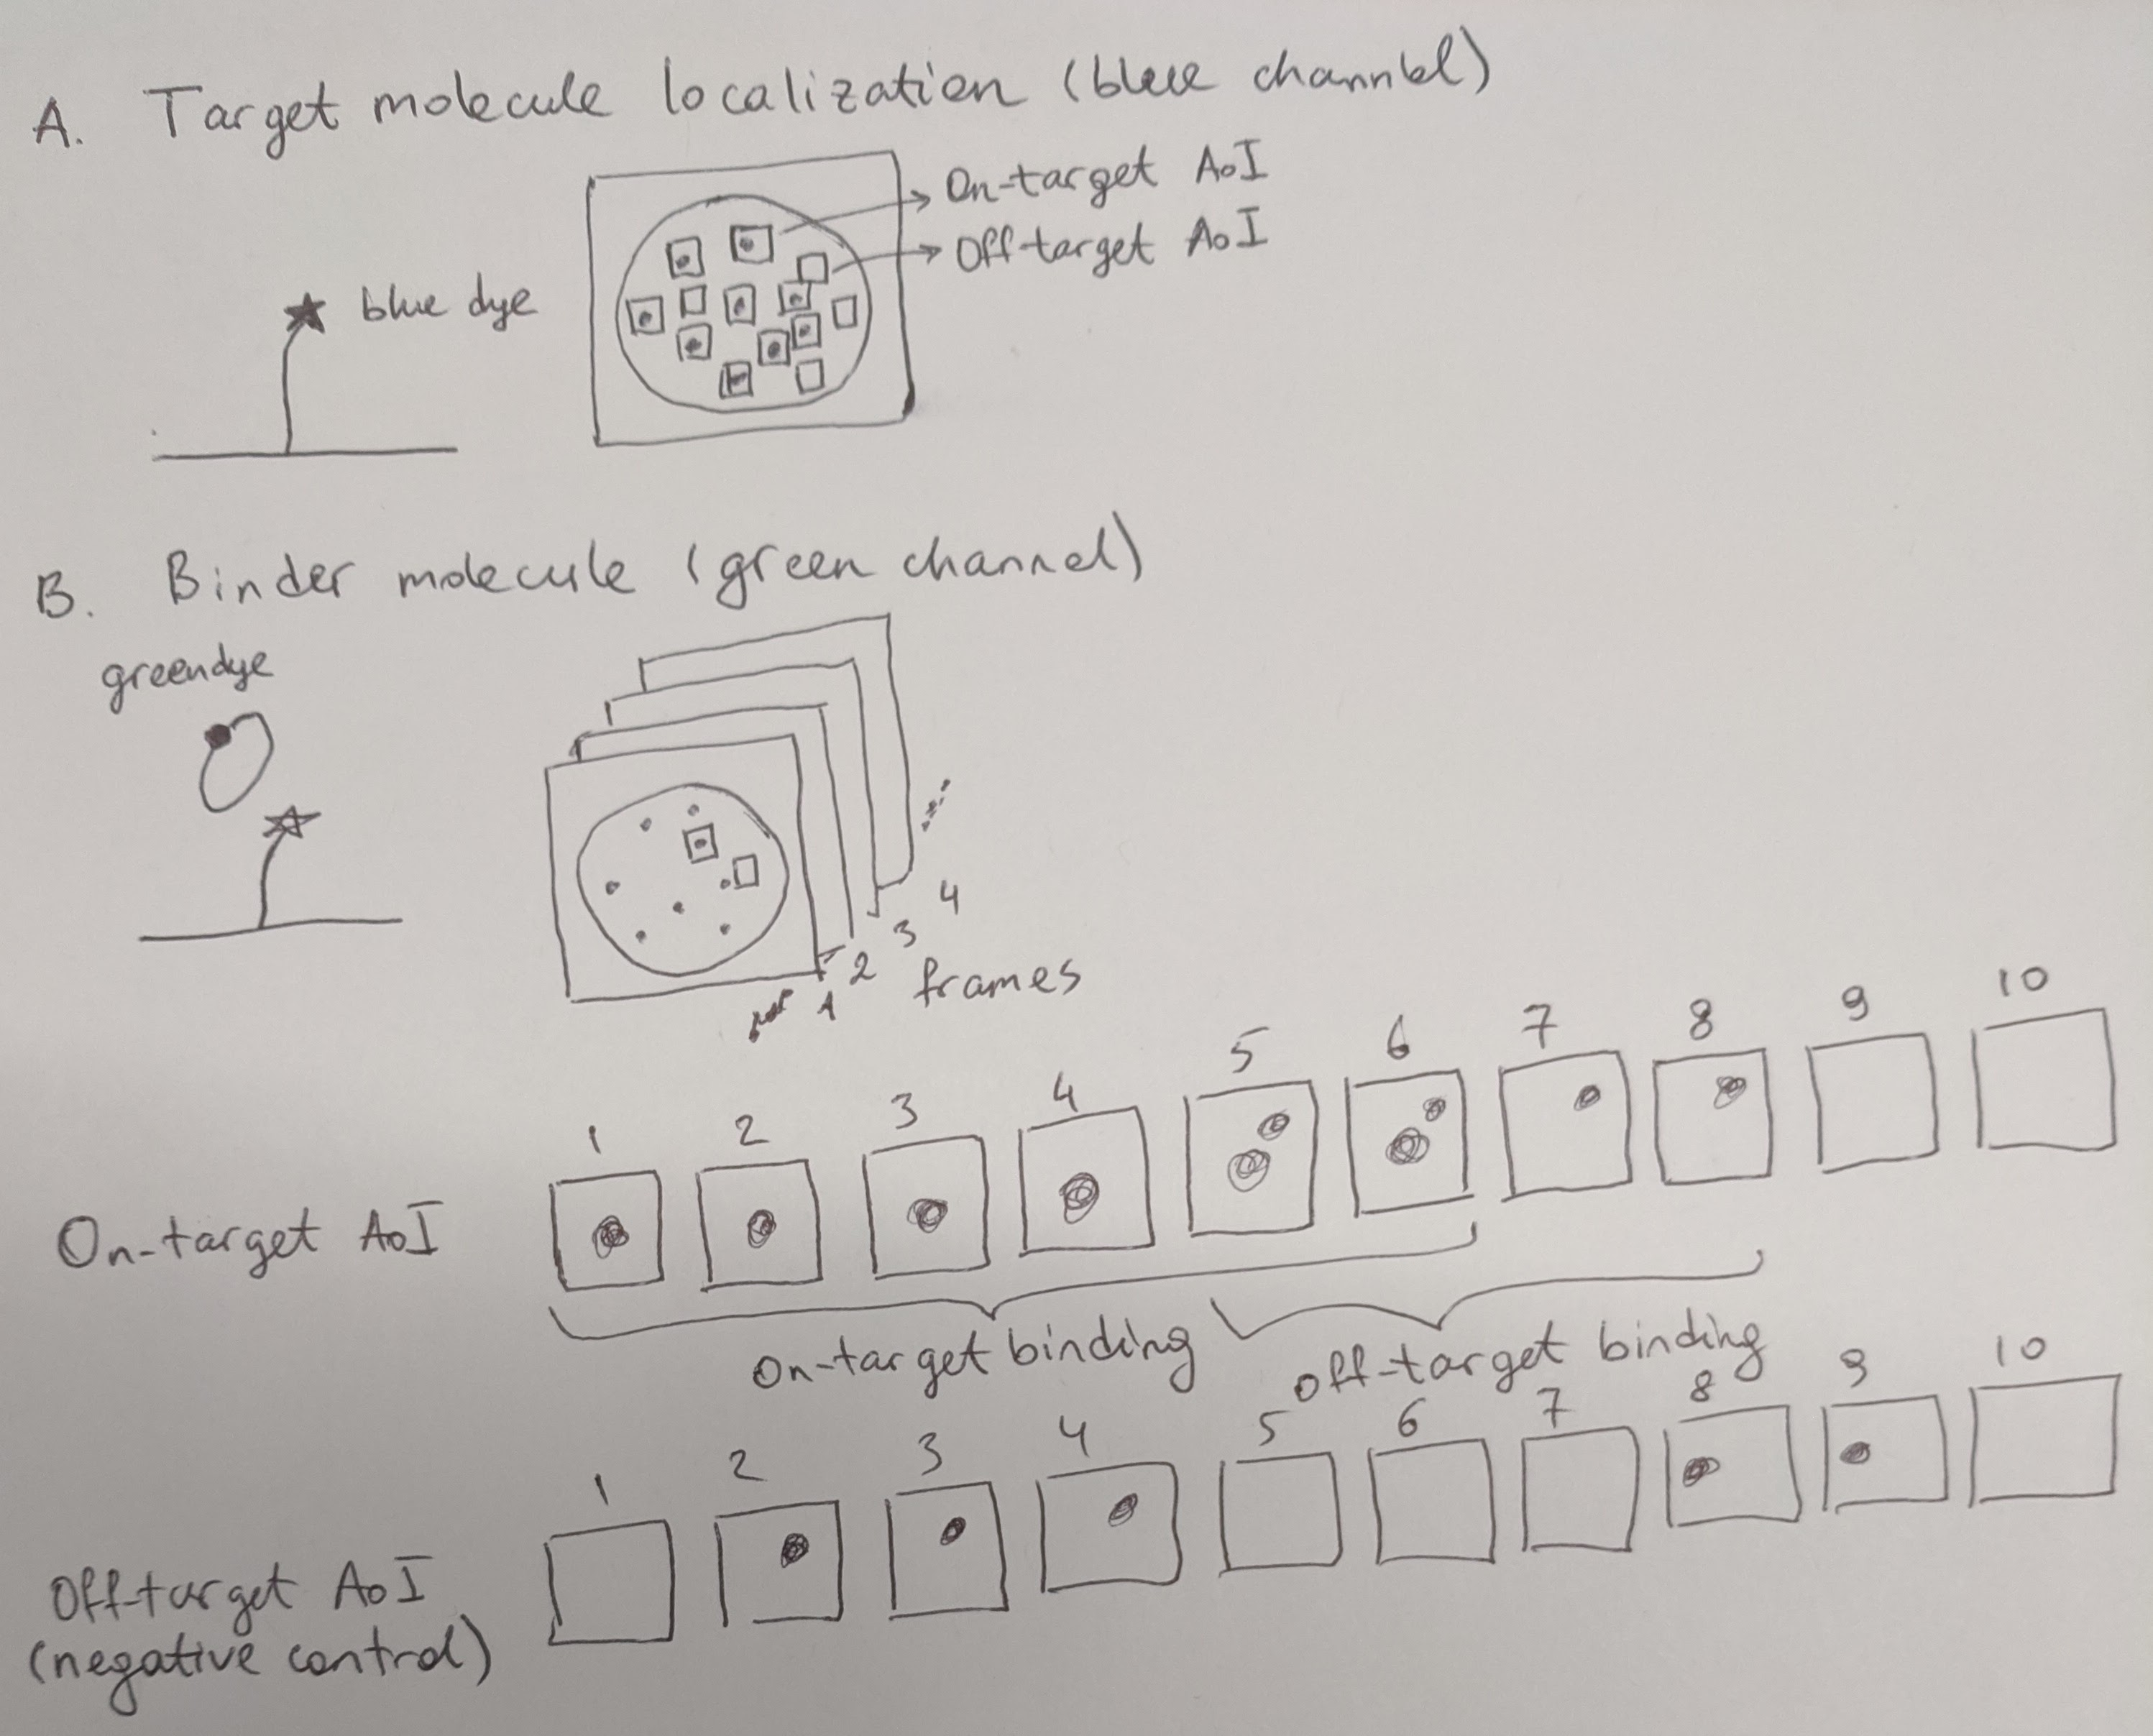
\includegraphics[width=\linewidth]{figures/figure1.jpg}
%\caption{Co-localization single molecule spectroscopy experiment. (A) Target molecules are localized in the blue channel and then on-target and off-target areas of interest are selected. (B) Movies of the binder molecule collected in the green channel. In selected AoI binder molecules can be on-target, off-target, or absent.}
%\label{fig:cosmos_experiment}
%% If the optional argument in the square brackets is "none", then the caption *will not appear in the main figure at all* and only the full caption will appear under the supplementary figure at the end of the manuscript.
%\figsupp[Shorter caption for main text.]{This is a supplementary figure's full caption, which will be used at the end of the manuscript.}{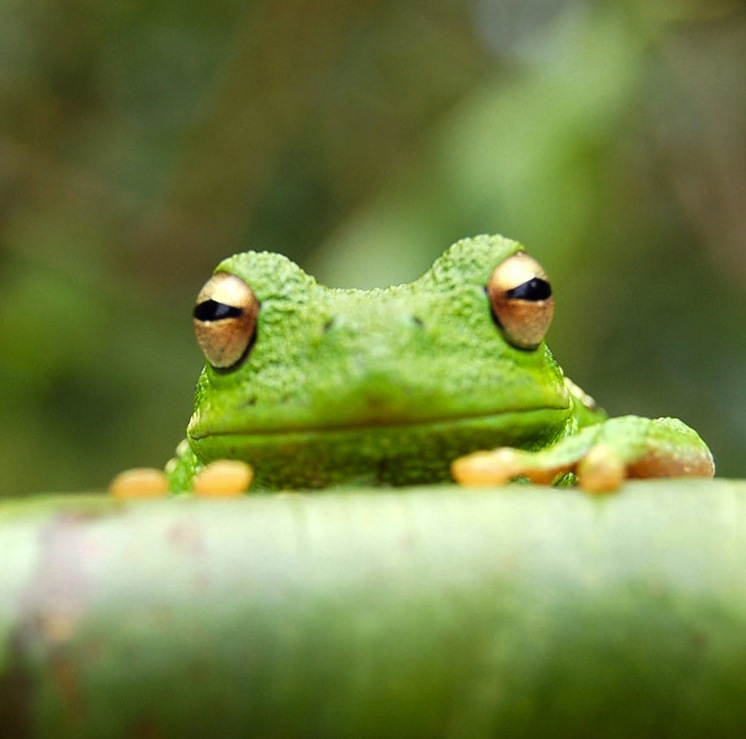
\includegraphics[width=6cm]{frog}}\label{figsupp:sf1}
%\figsupp{This is another supplementary figure.}{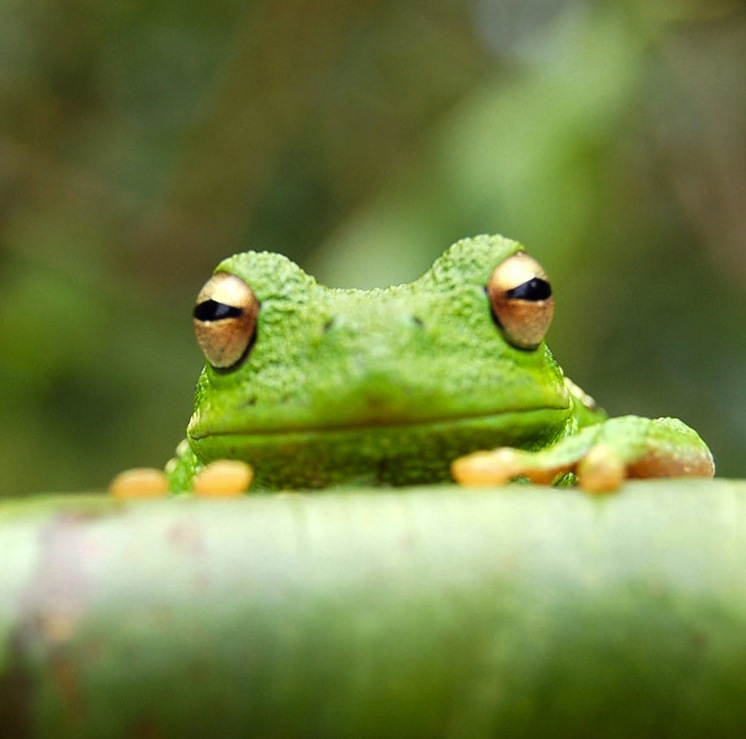
\includegraphics[width=6cm]{frog}}
%\figdata{This is a description of a data source.}\label{figdata:first}
%\figdata{This is another description of a data source.}\label{figdata:second}
%\end{figure}

%\begin{figure}
%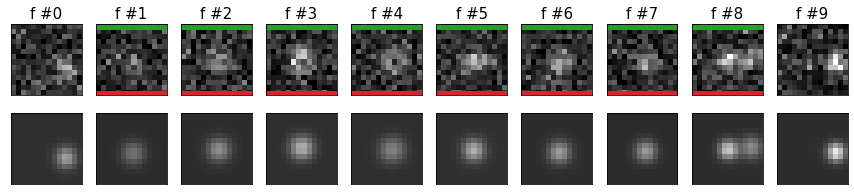
\includegraphics[width=\linewidth]{figures/figure3a.png}
%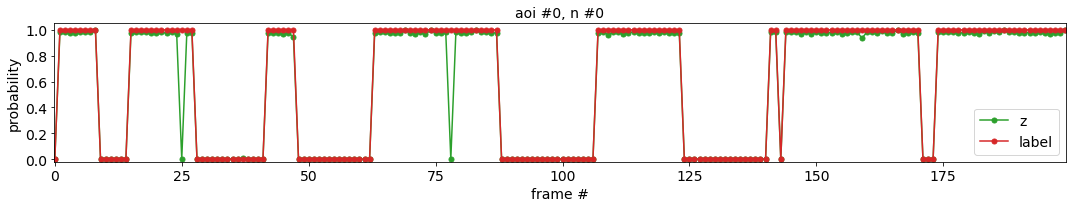
\includegraphics[width=\linewidth]{figures/figure3b.png}
%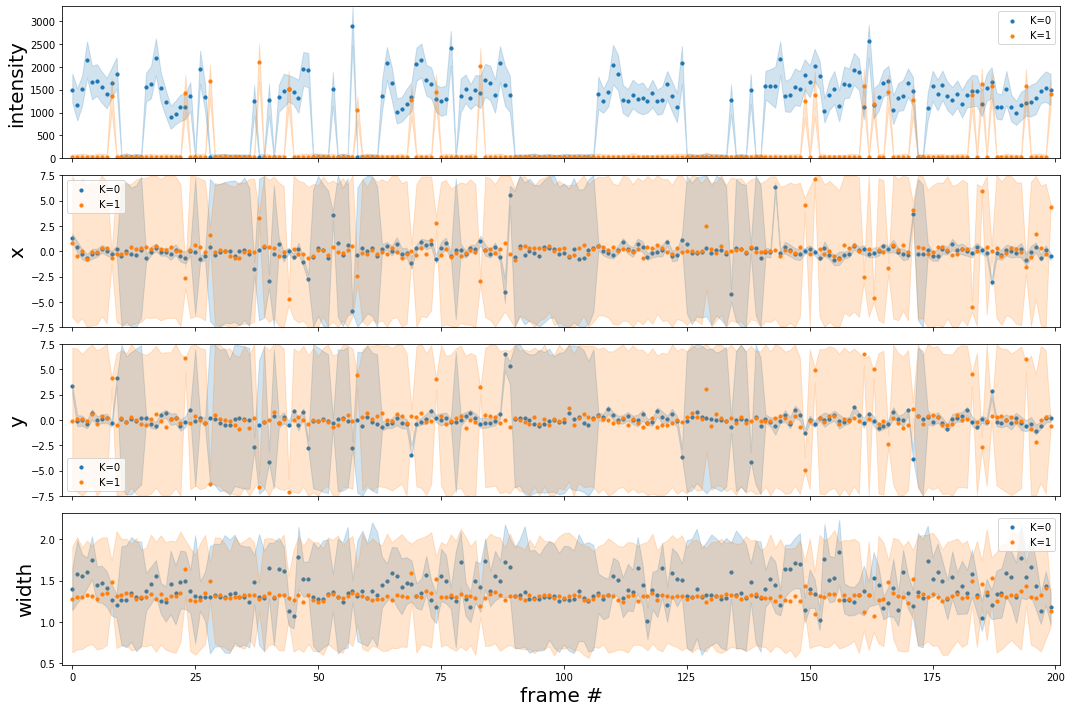
\includegraphics[width=\linewidth]{figures/figure3c.png}
%\caption{Co-localization single molecule spectroscopy experiment. (A) Target molecules are localized in the blue channel and then on-target and off-target areas of interest are selected. (B) Movies of the binder molecule collected in the green channel. In selected AoI binder molecules can be on-target, off-target, or absent.}
%\label{fig:view}
%\end{figure}